
\subsection{PN-Übergang \todo{5x}}\label{k5:pn}
    
    \subsubsection{Raumladungszone}\label{k5:rlz}
	Elektronen aus dem \textit{n}-dotierten Bereich diffundieren zum \textit{p}-dotierten Bereich was zu einer Elektronenverarmung der \textit{n}-seitigen Randzone führt. 
	Dadurch wird die \textit{n} Seite positiv aufgeladen. Umgekehrt kommt es zu einer Löcherverarmung auf der \textit{p} Seite und somit zu einer negativen Aufladung dort. 
    Dadurch entsteht am Übergang eine hochohmige Verarmungszone, die sogenannte \textit{Raumladungszone} (RLZ).
    Diese Raumladung erzeugt ein Feld, welches der weiteren Diffusion von Ladungsträgern entgegenwirkt. Das Maximum der elektrischen Feldstärke liegt an der \textit{pn}-Grenze (\ref{fig:raumladungszone} b).
    
    Durch dieses elektrische Feld entsteht eine Potenzialdifferenz welche auch als \textit{Diffusionsspannung} bezeichnet wird berechnet sich folgendermaßen berechnet:
    \begin{equation}
        U_D = \varphi_2 - \varphi_1 = \int{x_1}^{x_2} E \cdot dx
    \end{equation}

           \begin{figure}[H]
        \centering
        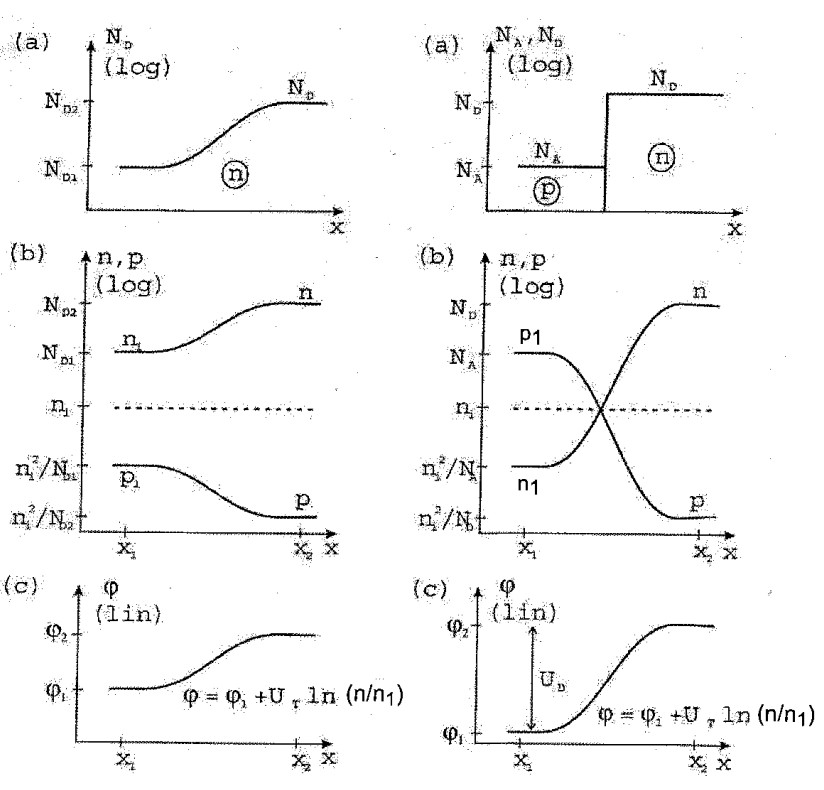
\includegraphics[width=0.5\textwidth]{fig/pnuebergang.jpg}
        \caption{linkes Bild: $nn^+$ -Übergang. Rechtes Bild: \textit{pn}-Übergang. (a) Dotierung (b) Ladungsträgerdichten (c) Potenzialverlauf}
        \label{fig:pnuebergang}
    \end{figure}
    
	$U_D$ in Silizium bei Zimmertemperatur beträgt ca. 0.8V 
    \begin{figure}[H]
        \centering
        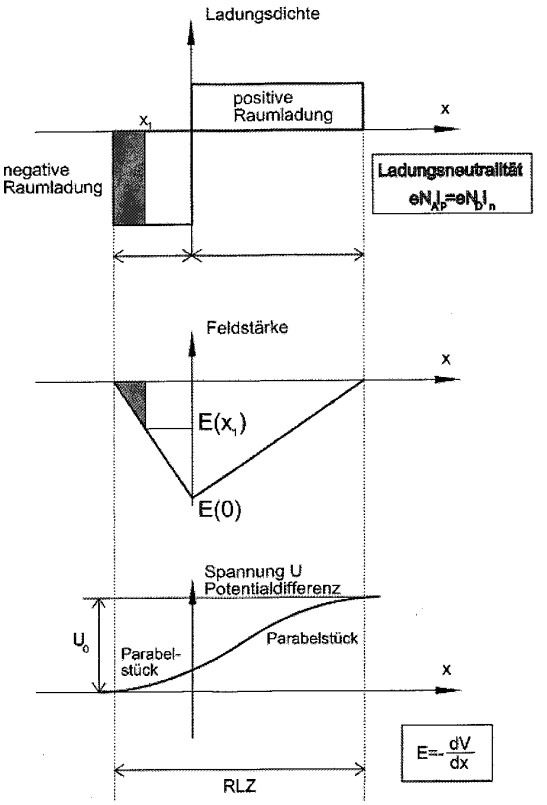
\includegraphics[width=0.5\textwidth]{fig/raumladungszone}
        \caption{Raumladungsdichte (a), Feldstärke (b) und Potenzial (c) am \textit{pn}-Übergang}
        \label{fig:raumladungszone}
    \end{figure}
    
       \begin{figure}[H]
        \centering
        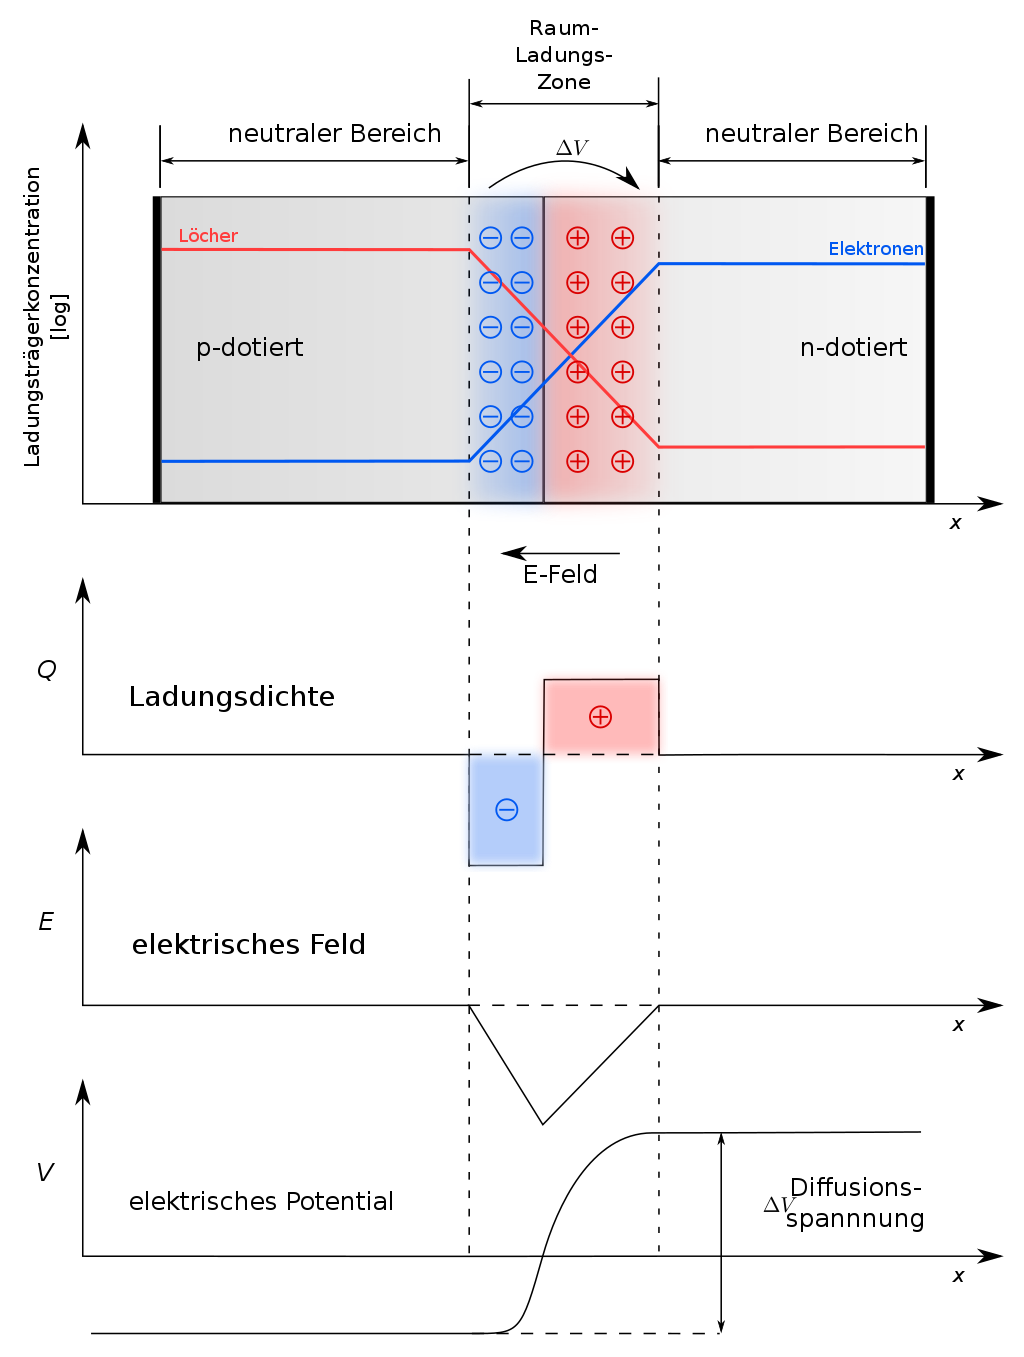
\includegraphics[width=0.5\textwidth]{fig/raumladungszone-wiki}
        \caption{Nochmal die Raumladungszone, diesmal von Wikipedia in Bunt und Farbe}
        \label{fig:raumladungszone-wiki}
    \end{figure}


	\subsubsection{Aufzeichnen ohne externe Spannung}
	Läuft wohl auf das darstellen der Raumladungszone und des elektrischen Feldes wie in \autoref{fig:raumladungszone-wiki} und \autoref{fig:raumladungszone} hinaus?
	Ohne externe Spannung kommt es wie oben beschrieben zur Ausbildung einer Raumladungszone. Bei dieser wandern die Elektronen aus dem n-Halbleiter zu den Löchern des p-Halbleiters und umgekehrt. Dabei entsteht eine Zone ohne freie Ladungsträger - eben die Raumladungszone. 
	
	\subsubsection{Diagramm dazu, wo auf x-Achse Ort (Verlauf von pn Übergang) und auf der y-Achse Dichte der freien Elektronen}
       \begin{figure}[H]
        \centering
        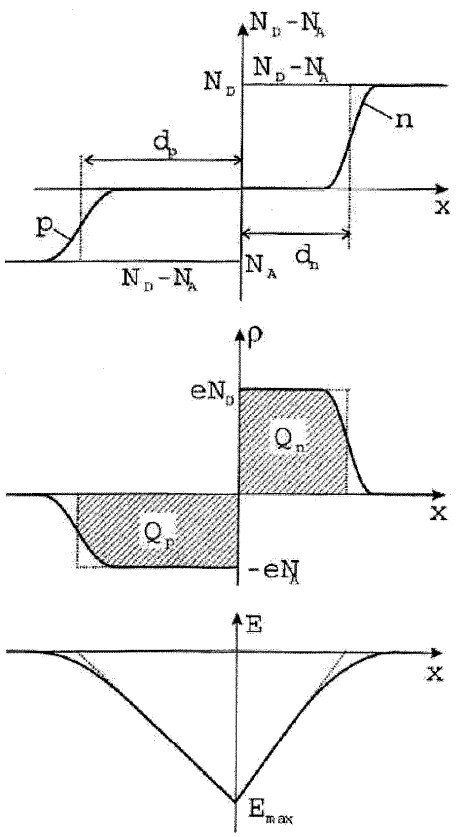
\includegraphics[width=0.5\textwidth]{fig/dotierungsVerlauf}
        \caption{Verlauf der Dotierung, der Trägerdichten \textit{n} und \textit{p}, der Raumladung $\rho$ und der Feldstärke E am abrupten \textit{pn}-Übergang. Beachten Sie, dass hier die Dichten linear aufgetragen sind.}
        \label{fig:dotierungsVerlauf}
    \end{figure}

	Hier kann man entweder mit \autoref{fig:raumladungszone-wiki} und \autoref{fig:raumladungszone} beginnen.
	Mehr Sinn macht es aber wahrscheinlich \autoref{fig:pnuebergang} aufzuzeichnen, oder sich auf \autoref{fig:dotierungsVerlauf} zu beziehen. 
	Dort kann man mit der Dotierung beginnen (diskreter Sprung, da p und n dotiert!) und die zweite Reihe stellt dann die Ladungsträgerdichte dar. Achtung, die Dichten sind logarithmisch angegeben!
	
	$N_A$ (p-Halbleiter) und $N_D$ (n-Halbleiter) stellen jeweils die Dotierungen dar, der Sprung stellt den Dotierungsverlauf / Übergang von p auf n dar.
	$n_i$ wird \textit{Intrinsic}-Zahl oder auch Eigenleitungsdichte genannt und beschreibt die Trägerdichte im undotierten Halbleiter und wird detailliert in Kapitel 3 diskutiert bzw. eingeführt. 
	
	Wikipedia hat dazu folgende Definition: Die Eigenleitungsdichte ist die charakterisierende Materialeigenschaft eines Halbleiters mit Blick auf seine elektrische Leitfähigkeit.
	Die Eigenleitungsdichte beschreibt den Mindestwert der elektrischen Leitfähigkeit, die tatsächliche Leitfähigkeit kann höher liegen (durch Verunreinigung, Dotierung). Diese Störstellenleitung (eben durch Dotierung) liegt üblicherweise um mehrere Größenordnungen über der Eigenleitung. 
	
	\subsubsection{Größenordnung einschätzen: Abstand von Elektronen, Größe von RLZ (normaler PN Übergang, Tunneldiode), Elektronendichte im HL}
	Ist eventuell in Kapitel 3 besprochen?
	
	\subsubsection{Skizze Flussrichtung, Sperrichtung, Raumladungszone}
	
	Wahrscheinlich ist hier die Darstellung des Bänderdiagramms gemeint, diese ist in \autoref{fig:pn-betriebszustände2}
	
       \begin{figure}[H]
        \centering
        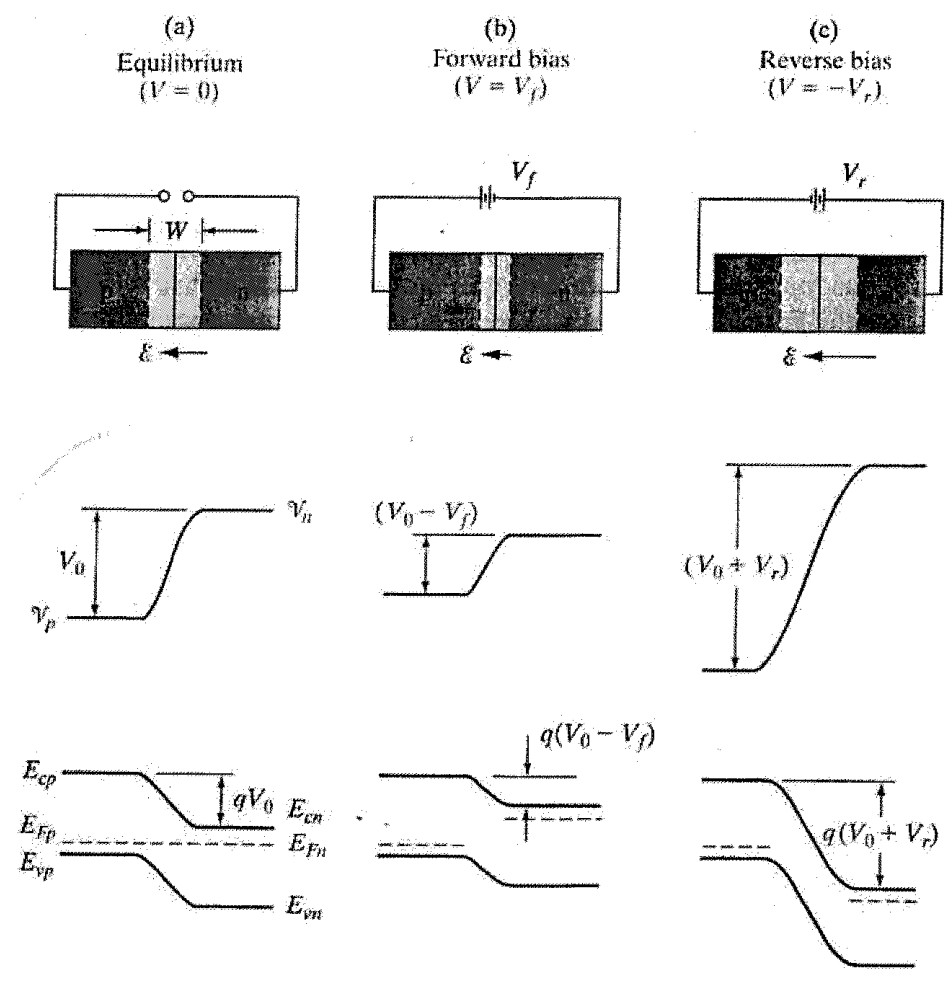
\includegraphics[width=0.5\textwidth]{fig/pn-fluss-sperr-rlz.jpg}
        \caption{Betriebszustände des pn-Übergangs (a) $U = 0$ (b) Flussrichtung $U = V_f$ (c) Sperrpolung $U = -V_r$, p-Zone negativ gegenüber n-Zone}
        \label{fig:pn-betriebszustände2}
    \end{figure}
	
    
       \begin{figure}[H]
        \centering
        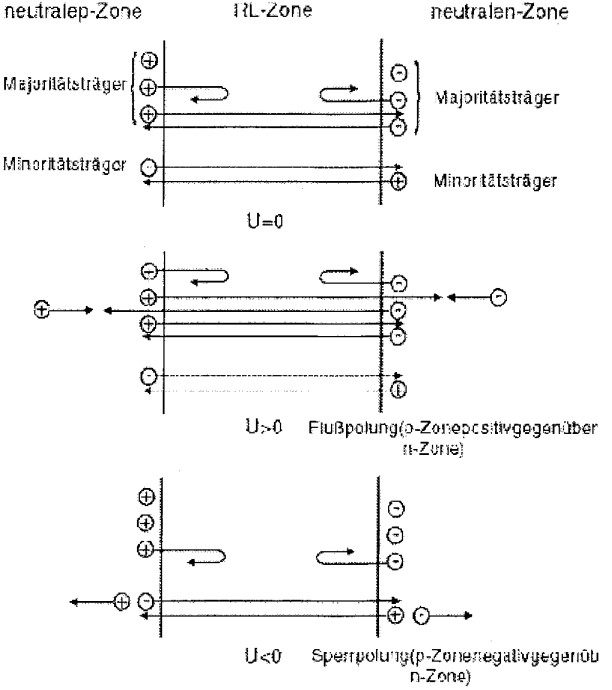
\includegraphics[width=0.5\textwidth]{fig/pn-betriebszustande}
        \caption{Betriebszustände des pn-Übergangs (oben) $U = 0$ (mitte) Flußpolung $U > 0$, p-Zone positiv gegenüber n-Zone (unten) Sperrpolung $U < 0$, p-Zone negativ gegenüber n-Zone}
        \label{fig:pn-betriebszustände}
    \end{figure}
    
    \subsubsection{Flussbetrieb}
    \emph{Noch einfachere Beschreibung (und korrekte)}: Bei Polung in Durchlassrichtung (+ am p-Kristall und - am n-Kristall) wird der Potentialwall abgebaut. Das elektrische Feld der Sperrschicht wird aber einer gewissen angelegten Spannun gkomplett neutralisiert und es ergibt sich mit dem von außen angelegten elktrischen Feld ein neues elektrisches Feld, welches Ladungstransport durch den gesamten Kristall erlaubt. Neue Ladungsträger fließen von der äußeren Quelle auf die Sperrschicht zu und rekombinieren hier fortwährend. Bei ausreichender angelegter Spannung fließein signifikanter elektrischer Strom.
    Das Skriptum hat dazu noch \autoref{fig:pn-flussbetrieb} zu bieten.
    
    \emph{Vereinfachte Beschreibung}: Legt man eine äußere Spannung U an, sodass das p-Gebiet gegenüber dem n-Gebiet positiver wird, so werden die Löcher auf die n-Seite und die Elektronen auf die p-Seite getrieben.
    
    \emph{Korrekte Beschreibung}: Die äußere Spannung U kann wegen der hohen Ladungsträgerdichten in den neutralen Zonen nur in der Raumladungszone abfallen. Sie verringert dort die Diffusionsspannung von $U_D$ (in Silizium 0.7V) auf $U_D-U$. 
    
    Elektronen und Löcher können nun wieder vermehrt durch Diffusion zur pn-Grenze wandern. Die Raumaldungszone wird mit beweglichen Ladungsträgern zugeschüttet und die Diode leitet. 
    
    Wegen der Verringerung der Potentialbarriere und des exponentiellen Verlaufes der Energieverteilung der Elektronen kommt es zu einer exponentiellen Abhängigkeit des Stromes von der Spannung (Exponentialkennlinie).
    
    \begin{figure}
        \centering
        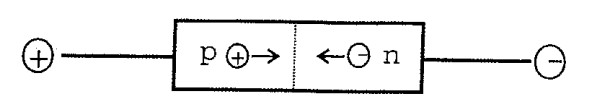
\includegraphics[width=0.33\textwidth]{fig/pn-flussbetrieb.jpg}
        \caption{Schematische Darstellung des Flussbetriebs}
        \label{fig:pn-flussbetrieb}
    \end{figure}
    
    \subsubsection{Sperrterieb}
    Durch Anlegen einer äußeren Spannung in Sperrichtung (+ am n-Kristall, - am p-Kristall) wird das elektrische Feld der Sperrschicht verstärkt und die Ausdehnung der Raumladungszone vergrößert. Elektronen und Löcher werden von der Sperrschicht weggezogen. Es fließt nur ein sehr geringer Strom, erzeugt durch Minoritätsladungsträger (Sperrstrom), außer die Durchbruchspannung wird überschritten.
    Aus dem Skriptum wieder: \autoref{fig:pn-sperrbetrieb}
    \begin{figure}
        \centering
        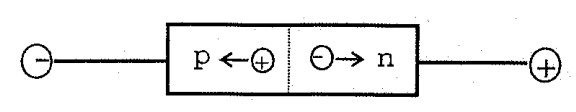
\includegraphics[width=0.33\textwidth]{fig/pn-sperrbetrieb.jpg}
        \caption{Schematische Darstellung des Sperrbetriebs}
        \label{fig:pn-sperrbetrieb}
    \end{figure}

	\subsubsection{Skalen, logarithmisch, linear, Größenordnung}
	\autoref{fig:dotierungsVerlauf} stellt die Raumladungszone linear dar, während \autoref{fig:pnuebergang} mit einer logarithmischen Darstellung arbeitet.
	Größenordungen werden wahrscheinlich wieder in Kapitel 3 erwähnt. 
	
	\subsubsection{Freie Elektronen}
	
	\subsubsection{Anzahl}
	\subsubsection{Dotierung}
	

	
\subsection{Diodenkennlinie \todo{0x}}\label{k5:diode}
Durch die Polung in Durchlassrichtung treibt die äußere Spannung sowohl die Elektronen aus dem n-Gebiet, als auch die Löcher aus dem p-Gebiet auf die Raumladungszone zu, die somit wieder bewegliche Ladungsträger enthält und ihre Sperrwirkung verliert. 
    \begin{figure}[H]
        \centering
        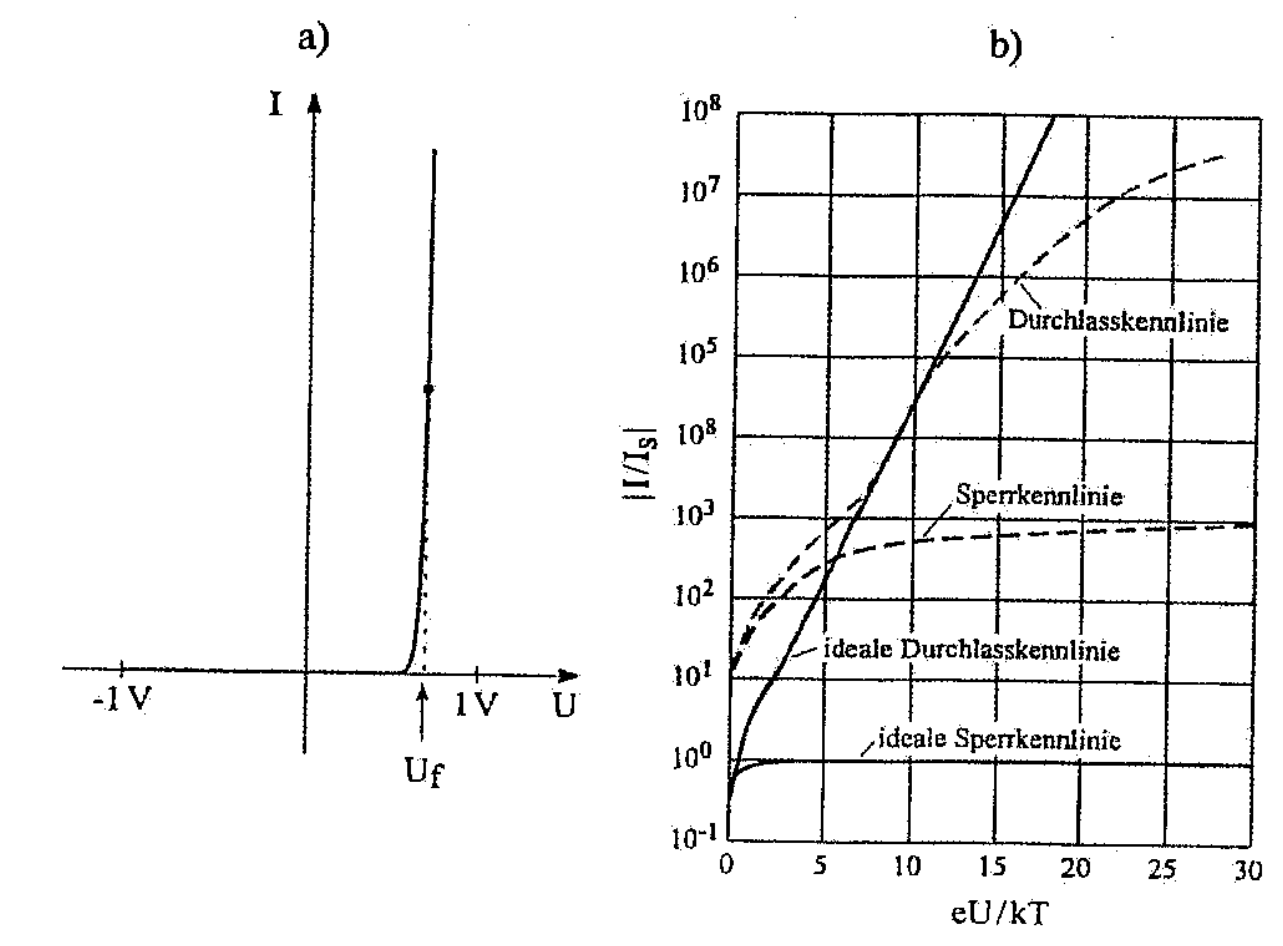
\includegraphics[width=0.8\textwidth]{fig/diodenkennlinie}
        \caption{(a) ideale Diodenkennlinie (linear), (b) ideale und nichtideale Kennlinie (logarithmisch)}
        \label{fig:diodenkennlinie}
    \end{figure}
    \subsubsection{Warum exponentiell?}
    Shockley-Gleichung in 2 Schritten:
    \begin{enumerate}
        \item Elektronenkonzentration am p-seitigen Rand der RLZ berechnen ( = L\"ocherkonzentration am p-seitigen Rand)
        \item Diffusion der Elektronen im neutralen p-Gebiet behandeln
    \end{enumerate}
    \begin{equation}
        I = I_S (e^{\frac{U_D}{n \cdot U_T}} - 1)
    \end{equation}
    Mit
    \begin{itemize}
        \item S\"attigungssperrstrom $I_S \approx 10^{-12} \ldots 10^{-6}A$
        \item Emissionskoeffizient $n \approx 1 \ldots 2$
        \item Temperaturspannung $U_T=\frac{k \cdot T}{q} \approx 25mV$ bei Raumtemperatur
        \item Temperatur $T$
        \item Boltzmannkonstante $k=1.381\cdot 10^{-23} Ws/K$
        \item Elementarladung $q = 1.602 \cdot 10^{-19}As$
    \end{itemize}
    \subsubsection{Verlauf der Kapazit\"at einer Diode als Funktion der Spannung}
    Der p-n \"Ubergang von Dioden hat eine Kapazit\"at, die von der Breite der RLZ abh\"angig ist. Mit steigender Sperrspannung vergr\"o{\ss}ert sich die Breite der ladungsfreien Zone, wodurch die Kapazit\"at abnimmt. Zu sehen in \Cref{fig:diodenkapazitaet} mit $m_s$ als Kapazit\"atskoeffizient, der das Dotierungsprofil darstellt.
    \begin{figure}
        \centering
        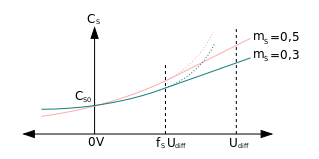
\includegraphics[width=0.5\textwidth]{fig/diodenkapazitaet}
        \caption{Sperrschichtkapazit\"at von Dioden}
        \label{fig:diodenkapazitaet}
    \end{figure}
    \subsubsection{Wie sehen die Ladungen bei anlegen einer Spannung aus?}
    Durch anlegen einer Spannung in Durchlassrichtung werden elektronen (aus dem n-Gebiet) und L\"ocher (aus dem p-Gebiet) in die RLZ getrieben. Die RLZ verschwindet und die Diode leitet.\\
    Bei anlegen einer Spannung in Sperrrichtung werden die Elektronen und L\"ocher noch weiter auseinandergetrieben, die RLZ wird gr\"o{\ss}er, die Diode sperrt.
    \subsubsection{Massenwirkungsgesetz}
    Siehe \Cref{k3:kontinuitaet}.

\subsection{Banddiagramm für PN ohne Spannung \todo{1x}}\label{k5:pnBand}
Siehe \Cref{fig:pn-banddiagramm}.
\begin{figure}[H]
    \centering
    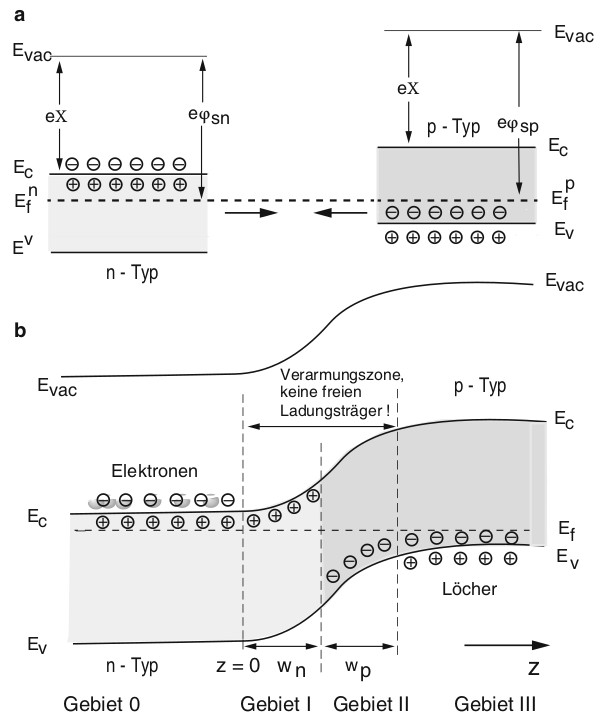
\includegraphics[width=0.66\textwidth]{fig/pn-bandstruktur.jpg}
    \caption{Formation eines pn-Übergangs. a Die p- und n-Gebiete vor der Formation des Über-
gangs. Im p-Gebiet liegt das Fermi-Niveau knapp oberhalb der Valenzbandkante, im n-Gebiet
knapp unterhalb des Leitungsbandes. Die Elektronenaffinitäten $e_\xi$ und Austrittsarbeiten $e\Phi_{sp}$
und $e\Phi_{sn}$ , sowie das Fermi-Niveau sind ebenfalls eingezeichnet. b Bandprofil des fertigen
pn-Übergangs inklusive Vakuumniveau. Die Bandlücke ist überall die gleiche und, wichtig, Va-
lenzband und Leitungsband verlaufen immer parallel.}
    \label{fig:pn-banddiagramm}
\end{figure}

\begin{figure}
    \centering
    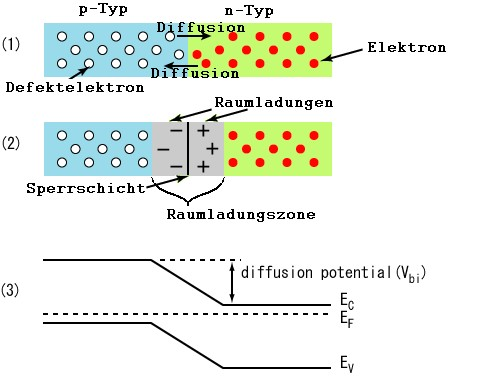
\includegraphics[width=0.66\textwidth]{fig/pn-banddiagramm2}
    \caption{Nochmal die selbe Darstellung mit bereits zusammengefügtem PN-Übergang.}
    \label{fig:pn-banddiagramm}
\end{figure}

\subsection{Schottky-Kontakt-Diode \todo{0x}}\label{k5:schottky}
Schottky-Dioden werden aus einem Metall-Halbleiter Kontakt gebaut. Dies geschieht implizit bei jedem Kontakt von Transistoren und Dioden und hat dementsprechend hohe Wichtigkeit.
Die Schottky-Diode besteht aus einer Metall-Schicht und z.B. einer n-leitenden Silizium-Schicht. Die Elektronen der n-Schicht wandern zur Metallschicht. Weil Elektronen leichter aus n-Silizium in die Metallschicht gelangen als umgekehrt, entsteht in der Silizium-Schicht ein an Elektronen verarmter Bereich, die sogenannte Schottky-Sperrschicht. Durch die Ladungsträgerdiffusion entsteht eine Raumladungszone (Sperrschicht) und ein elektrisches Feld. Ab einem bestimmten Zustand ist das elektrische Feld so groß, dass keine Elektronen mehr wandern.
Schaltet man die Schottky-Diode in Sperrrichtung - Plus an n-Silizium und Minus an die Metallschicht - dann wird die Raumladungszone größer. Sie nimmt einen großen Bereich des n-Siliziums ein. Schaltet man die Schottky-Diode in Durchlassrichtung, wird die Raumladungszone freigeräumt. Die Elektronen fließen von der n-Schicht in die Metallschicht.
Das Schalten vom Durchlasszustand in den Sperrzustand bzw. umgekehrt erfolgt sehr schnell. Es müssen keine Minderheitsladungsträger ausgeräumt werden. Der Strom durch die Schottky-Diode besteht daher nur aus Elektronen.
\begin{figure}[h]
    \centering
    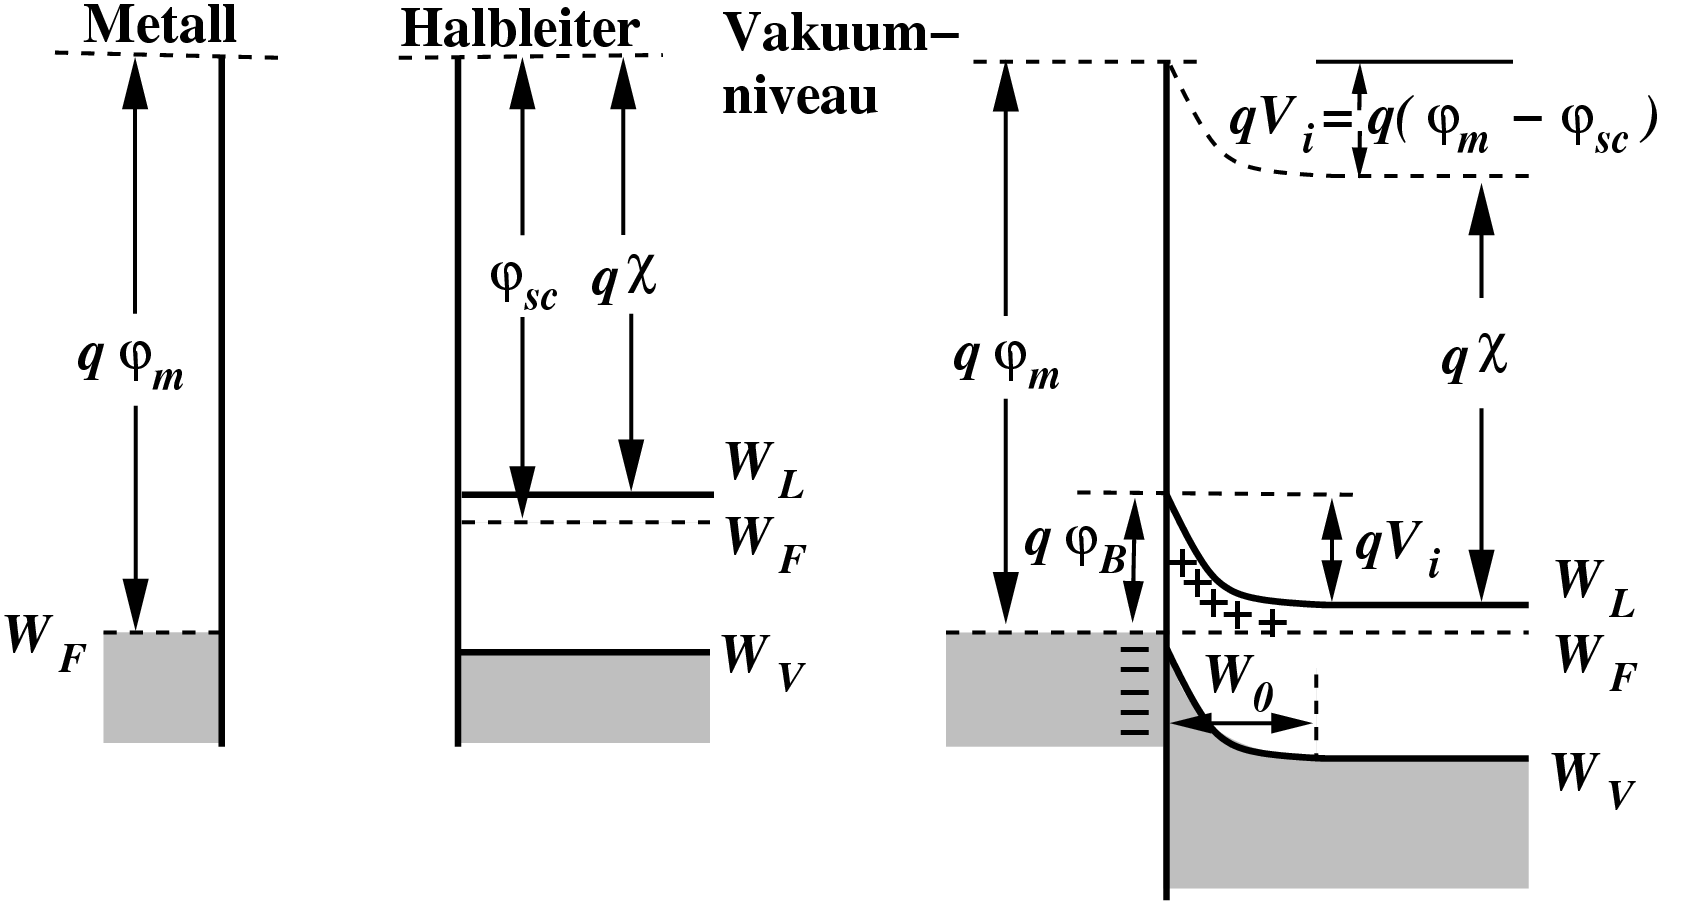
\includegraphics[width=0.75\textwidth]{fig/baenderSchottky}
    \caption{Baenderdiagramm vor und nach dem zusammenlegen von Halbleiter und Metall}
    \label{fig:baenderSchottky}
\end{figure}

\subsection{Tunneldiode \todo{4x}}\label{k5:tunnelDiode}
Die Tunneldiode hat ein hochdotiertes n-leitendes Germanium-Plättchen in das eine ebenfalls hochdotierte Indium-Pille einlegiert ist.
Wegen der hohen Dotierung wirkt die Sperrschicht nicht. Die Sperrschicht wird durch die Elektronen mit hoher Geschwindigkeit durchtunnelt. Die Elektronen durchfliegen nahezu mit Lichtgeschwindigkeit diesen Tunnel. Schon bei einer kleinen Durchlassspannung fließt ein Strom, obwohl die Sperrschicht noch nicht abgebaut ist.

In \Cref{fig:tunneldiode0V} sieht man wie die hohe dotierung zu einer Verschiebung des Fermi-Niveaus ins Leitungs- bzw. Valenzband f\"uhrt.
    \begin{figure}[H]
        \centering
        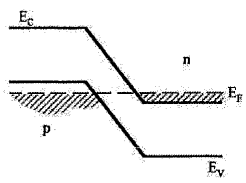
\includegraphics[width=0.4\textwidth]{fig/tunneldiode0V}
        \caption{Banddiagramm der Tunneldiode ohne externe Spannung}
        \label{fig:tunneldiode0V}
    \end{figure}
In \Cref{fig:tunneldiodeFlusspolung} werden schon durch eine kleine Spannung die Energieb\"ander der n-Seite
so weit nach oben verschoben, dass die Elektronen des Leitungsbandes in die leeren Zust\"ande am oberen Ende des Valenzbandes tunneln k\"onnen. Wo das maximum dieses Stroms liegt ist von der Fl\"ache der pn-Zone abh\"angig (typisch $\approx 100mV$).\\
Wird die Spannung gr\"oßer, steht den Leitungselektronen der n-Seite das verbotene Band der p-Seite gegen\"uber.
In diesem Abschnitt hat die Diode einen negativen differentiellen Widerstand, der zur Schwingungserzeugung
und Verst\"arkung genutz werden kann.\\
Bei noch gr\"oßerer Spannung setzt dann der normale Diffusionsstrom ein.
    \begin{figure}[H]
        \centering
        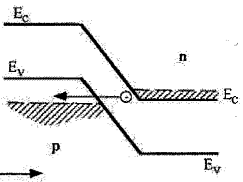
\includegraphics[width=0.4\textwidth]{fig/tunneldiodeFlusspolung}
        \caption{Banddiagramm der Tunneldiode mit Polung in Flussrichtung}
        \label{fig:tunneldiodeFlusspolung}
    \end{figure}
In \Cref{fig:tunneldiodeSperrpolung} ist die Tunneldiode in Sperrrichtung gepolt abgebildet.
    \begin{figure}[H]
        \centering
        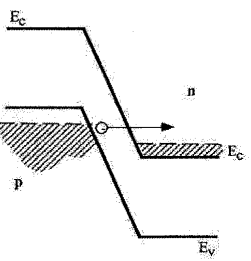
\includegraphics[width=0.4\textwidth]{fig/tunneldiodeSperrpolung}
        \caption{Banddiagramm der Tunneldiode mit Polung in Sperrrichtung}
        \label{fig:tunneldiodeSperrpolung}
    \end{figure}
    
    \subsubsection{Banddiagramm ohne externe Spannung}
    Siehe \Cref{fig:tunneldiode0V}
    \subsubsection{was passiert, wenn 25mV in Flussrichtung angelegt werden?}
    Es wird getunnelt (Siehe \Cref{fig:tunneldiodeFlusspolung})
    \subsubsection{im Banddiagramm Konstellation aufzeichnen, wo Maximum und Minimum in Kennlinie auftreten}
    Maximum in \Cref{fig:tunneldiodeFlusspolung}. F\"ur minimum die B\"ander des n-Bereichs so weit rauf zeichnen
    dass es dem Verbotenen Bereich des p-Bereichs gegen\"ubersteht.
    \subsubsection{Dicke Raumladungszone Dotierung}
    ???
    \subsubsection{Wie groß ist die Bandlücke in Volt}
    ???
    \subsubsection{Kennlinie der Tunneldiode}
    Siehe \Cref{fig:tunneldiodeKennlinie}.\\
    Merkmale:
    \begin{itemize}
        \item Keine Sperrfunktion
        \item Auch bei kleinen Spannungen wird durchgeschalten
        \item Es gibt einen Bereich mit negativem Widerstand
    \end{itemize}
    \begin{figure}[h]
        \centering
        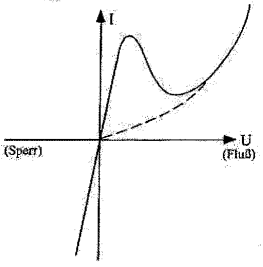
\includegraphics[width=0.75\textwidth]{fig/tunneldiode}
        \caption{Kennlinie der Tunnel-Diode}
        \label{fig:tunneldiodeKennlinie}
    \end{figure}
    
    \subsubsection{Kennlinie einer normalen Diode}
    Siehe \Cref{k5:diode}.

\subsection{Backward-Diode \todo{0x}}\label{k5:backward}
Die Backward-Diode ist eine Tunneldiode mit schw\"acherer Dotierung. Das Strommaximum und der fallende Ast
auf der Flu{\ss}seite verschwinden, es bleibt nur der steile Stromanstieg in Sperrrichtung \"ubrig.
Die starke Nichtlinearit\"at wird zur Gleichrichtung schwacher Signale und zur Mischung im Mikrowellenbereich
genutzt.

\subsection{Heterostrukturen \todo{0x}}\label{k5:heterostrukturen}

Zwei Halbleiter aus verschiedenen Materialien (z.B. GaAs und AlAs) nennt man Heterostrukturen.
Dies funktioniert nur wenn die Gitterkonstante ähnlich ist, die Bandlücken und Elektronenaffinitäten der beiden
Materialien können aber sehr verschieden sein.
Ähnlich zum pn-Übergang kommt es zum angleichen der Fermi-Niveaus und zu Band-Bending.
Da die Bandbreiten und Elektronenaffinitäten aber unterschiedlich sind, kommt es zu diskontinuitäten am Übergang
(\Cref{fig:heteroBand}).
\begin{figure}[h]
    \centering
    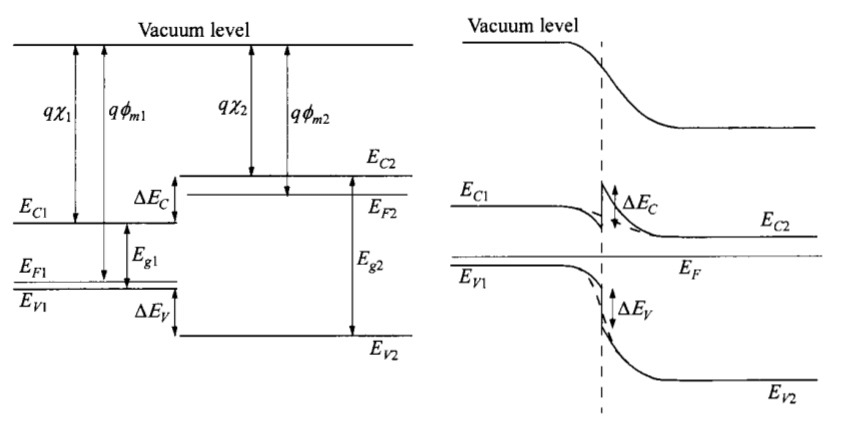
\includegraphics[width=0.75\textwidth]{fig/heteroBand}
    \caption{Banddiagramm einer Heterostruktur}
    \label{fig:heteroBand}
\end{figure}

Man unterscheidet Typ-I und Typ-II Heterostrukturen (\Cref{fig:heteroUnterschied}).
\begin{figure}[h]
    \centering
    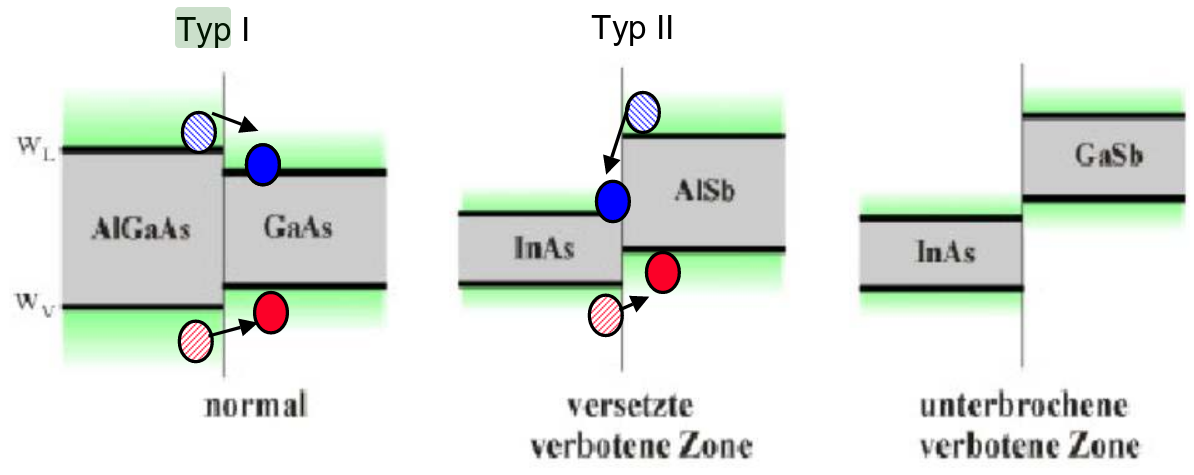
\includegraphics[width=0.75\textwidth]{fig/heteroUnterschied}
    \caption{Typ-I und Typ-II Heterostrukturen}
    \label{fig:heteroUnterschied}
\end{figure}

Heterostrukturen haben ideale Eigenschaften für optische Anwendungen.
Der Trick dabei ist, dass die Elektronen und Löcher in den vom GaAs
gebildeten Potentialtopf fallen und dort nicht wieder herauskommen. Auf diese
Weise erzwingt man lokal hohe Trägerdichten und damit eine hohe strahlende
Rekombinationsrate. Bei passenden äußeren optischen Bedingungen lässt sich
so auf einfache Weise eine Laseraktivität erzeugen.
Weitere Anwendungsbereiche: Kamerachips, schnelle GaAs-AlGaAs Feldeffekttransistoren,
Silizium Hetero-Bipolar-Transistor (höhere Geschwindigkeiten und bessere Stromverstärkung).
